\documentclass[dvipdfmx,autodetect-engine,titlepage]{jsarticle}
\usepackage[dvipdfm]{graphicx}
\usepackage{ascmac}
\usepackage{fancybox}
\usepackage{listings}
\usepackage{plistings}
\usepackage{itembkbx}
\usepackage{amsmath}
\usepackage{url}
\usepackage{graphics}
\usepackage{here}

\lstset{
  basicstyle={\ttfamily},
  identifierstyle={\small},
  commentstyle={\smallitshape},
  keywordstyle={\small\bfseries},
  ndkeywordstyle={\small},
  stringstyle={\small\ttfamily},
  frame={tb},
  breaklines=true,
  columns=[l]{fullflexible},
  numbers=left,
  xrightmargin=0zw,
  xleftmargin=3zw,
  numberstyle={\scriptsize},
  stepnumber=1,
  numbersep=1zw,
  lineskip=-0.5ex
}

\textheight=23cm
\renewcommand{\figurename}{図}
\renewcommand{\tablename}{表}
\newenvironment{code}
{\vspace{0.5zw}\VerbatimEnvironment  \begin{screen} 
\baselineskip=1.0\normalbaselineskip
 \begin{Verbatim}}
{\end{Verbatim}
\baselineskip=\normalbaselineskip
 \end{screen}\vspace{0.5zw}} 

\title{ワイヤレス通信システム(B1)\\
7th Week 伝送線路\\
}
\author{2600200087-2\\Oku Wakana\\奥 若菜}
\date{Jun. 12 2022}

\begin{document}

\maketitle

\section{給電線とアンテナの整合}
教科書32ページの図3.4のグラフをMATLABを用いて描画した。その際のソースコードを下に、得られたグラフを図1に示す。\\

\begin{lstlisting}[caption=ソースコード,label=1]
  figure

  % VSWRが1から10の範囲
  S = linspace(1,10);
  
  % VSWRから反射損Mを求める
  M = pow2db((1+S).^2./(4.*S));
  
  % VSWRが1,2,3...10のとき
  VSWR = 1:1:10;
  % それぞれの値の反射係数Gを有効数字小数点以下2ケタで求める
  G = round((VSWR-1) ./ (1+VSWR),2);
  
  % グラフのラインを引く
  line(S,M,'Color','r')
  
  %ラベル
  xlabel('VSWR')
  ylabel('\it M \rm[dB]')
  
  ax1 = gca; 
  ax1_pos = ax1.Position; 
  
  %反射係数Gのメモリをグラフ上部に表示する
  scale = 0:1/9:1;
  ax2 = axes('Position',ax1_pos,...
      'XAxisLocation','top',...
      'YTick', [], 'YTickLabel', {''}, ...
      'XTickLabelMode', 'manual', 'XTickMode', 'manual', ...  
      'XTick', scale, 'XTickLabel', cellstr(string(G)), ...
      'Color','none');
  
  %ラベル
  xlabel('|\Gamma|')
  
\end{lstlisting}

\begin{figure}[H]
  \centering
  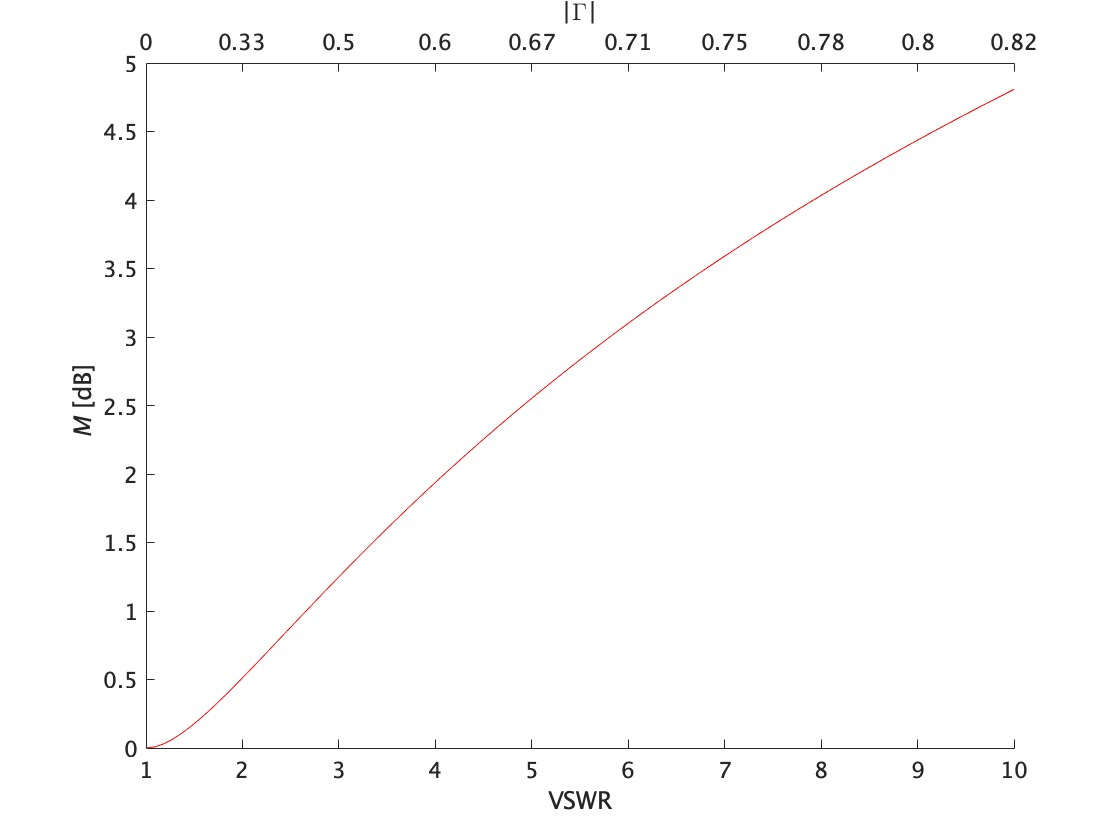
\includegraphics[scale=0.3]{f1.jpg}
  \caption{VSWRおよび反射係数と反射損の関係}\label{fig:図1}
\end{figure}

\end{document}
